% !TeX spellcheck = es_ES
\section{Lista 1}
\begin{enumerate}
    \item Demuestre que :
        \begin{enumerate}
            \item $\binom{n}{r} = \frac{n-r+1}{r}\binom{n}{r-1}$
            \begin{proof}
                \begin{align*}
                    \binom{n}{r} &= \frac{n!}{(n-r)!r!}\\
                    &= \frac{n-r+1}{n-r+1}(\frac{n!}{(n-r)!r!})\\
                    &= \frac{n-r+1}{n-r+1}(\frac{n!}{(n-r)!r(r-1)!})\\
                    &= \frac{n-r+1}{r}(\frac{n!}{(n-r+1)(n-r)!(r-1)!})\\
                    &= \frac{n-r+1}{r}(\frac{n!}{(n-r+1)!(r-1)!})\\
                    &= \frac{n-r+1}{r}(\frac{n!}{(n-(r-1))!(r-1)!})  \\
                    &= \frac{n-r+1}{r}\binom{n}{r-1}
                \end{align*}
            \end{proof}
            \item $(x+y)^n =\sum_{r=0}^{n} \binom{n}{r} x^{n-r}y^{r}$
            \begin{proof}
                Probemos para n=1
                \begin{gather*}
                (x+y)^1 = \sum_{r=0}^{1} \binom{n}{r} x^{n-r}y^{r}=  \binom{1}{0}(x^1)(y^0) + \binom{1}{1}(x^0)(y^1)= x + y =(x+y)^1 
                \end{gather*}\\  
                Supongamos 
                \begin{gather*}  
                (x+y)^n =   \sum_{r=0}^{n} \binom{n}{r} x^{n-r}y^{r}
                \end{gather*}
                Y probemos para $n+1$
                \begin{gather*}
                (x+y)^{n+1} = \sum_{r=0}^{n+1} \binom{n+1}{r} x^{n+1-r}y^{r}\\\
                \end{gather*}    
                \begin{align*}
                (x+y)^{n+1} &= (x+y)(x+y)^n = (x+y) \sum_{r=0}^{n+1} \binom{n}{r} x^{n-r}y^{r}\\
                &=x \sum_{r=0}^{n} \binom{n}{r} x^{n-r}y^{r} +  y \sum_{r=0}^{n} \binom{n}{r} x^{n-r}y^{r}\\
                &=\sum_{r=0}^{n} \binom{n}{r} x^{(n-1)-r}y^{r} +  y \sum_{r=1}^{n+1} \binom{n}{r-1} x^{n-(r-1)}y^{r}\\
                &=\binom{n}{0} x^{n+1}y^{0} + \sum_{r=1}^{n} \binom{n}{r} x^{(n+1)-r}y^{r} \\
                &+ \sum_{r=1}^{n} \binom{n}{r-1} x^{(n+1)-r}y^{r} + \binom{n}{n+r-1} x^{n-(r-1)}y^{n+1}\\
                &=x^{n+1} + \sum_{r=1}^{n} \binom{n}{r} x^{(n+1)-r}y^{r} +\sum_{r=1}^{n} \binom{n}{r-1} x^{n+1-r)}y^{r} + y^{n+1}\\
                &=x^{n+1} + \sum_{r=1}^{n} (\binom{n}{r} + \binom{n}{r-1}) x^{(n+1)-r}y^{r}+y^{n+1}\\
                &=x^{n+1}+\sum_{r=1}^{n} \binom{n+1}{r} (x^{(n+1)-r} y^r)\\
                &=\sum_{r=0}^{n+1} \binom{n+1}{r} (x^{(n+1)-r} y^r) \\
                \end{align*}
            \end{proof}
            \item $\sum_{r=0}^{n} r \binom{n}{r} = n2^{n-1} $
            \begin{proof}
                Tenemos que:
                \begin{gather*}
                {(1+x)}^n = \sum_{r=0}^{n} \binom{n}{r} (1^{n-r} x^r) =  \sum_{r=0}^{n} \binom{n}{r} x^r \\
                \end{gather*} Derivando: 
                \begin{gather*}
                n{(1+x)}^{n-1} = \sum_{r=1}^{n} r \binom{n}{r} {x^{r-1}} \
                \end{gather*} Y con x=1: 
                \begin{gather*}
                n2^{n-1} = \sum_{r=1}^{n} r \binom{n}{r} \\
                \end{gather*}
                \begin{gather*}
                \sum_{r=1}^{n} r \binom{n}{r} =  n2^{n-1} \\
                \end{gather*}
            \end{proof}
            \item $\sum_{r=0}^{n} \binom{n}{r} {(a-1)}^r = a^n $
            \begin{proof}
                \begin{gather*}
                a^n ={(a+1-1)}^n = {[1+(a-1)]}^n = \sum_{r=0}^{n} \binom{n}{r} (1^{n-r}) {(a-1)}^r\\
                \end{gather*}
                \begin{gather*}
                \sum_{r=0}^{n} \binom{n}{r} {(a-1)}^r = a^n\\
                \end{gather*}
            \end{proof}
            \item $ \sum_{r=0}^{n} {\binom{n}{r}}^2 =\binom{2n}{n} $
            \begin{proof}
                \begin{gather*}
                \sum_{r=0}^{n} {\binom{n}{r}}^2 =\binom{2n}{n}\\ 
                \end{gather*}
                \begin{gather*}
                {(1+x)}^{2n} = {(1+x)}^n * {(1+x)}^n = \sum_{r=0}^{n} (\sum_{r=0}^{n} \binom{n}{j} \binom{n}{r-j} x^k)\\ 
                \end{gather*}
                \begin{gather*}
                {(1+x)}^{2n} = \sum_{k=0}^{2n} \binom{2n}{k} x^k\\ 
                \end{gather*}
                \begin{gather*}
                \binom{2n}{n} = \sum_{j=0}^{n} \binom{n}{j} \binom{n}{n-j} = \sum_{j=0}^{n} {\binom{n}{j}}^2\\ 
                \end{gather*}
            \end{proof}
        \end{enumerate}
    \item ¿De cuantas maneras pueden formarse 5 personas para abordar un autobús, si dos de las personas se niegan a hacerlo una tras la otra?
    \item Dos focos se mantienen encendidos hasta que se funden. Suponer que ninguno dura mas de 1600 		horas. Definir un espacio muestral adecuado para este experimento, donde se describen los siguientes eventos:\\
    
    i)Ambos focos duran menos de 1000 horas     \\
    \textbf{Solucion}\\
    \begin{gather*}
    A = \lbrace x,y | 0\leq x,y <1000\rbrace \\
    \end{gather*}\\
    ii)Ningun foco se funde antes de 1000 horas 
    \\\textbf{Solucion}\\
    \begin{gather*}
    B = \lbrace x,y | 1000 < x,y \leq 1600\rbrace \\
    \end{gather*}\\
    iii) El menor tiempo de duracion (de los dos) es de 1000 horas
    \\\textbf{Solucion}\\
    \begin{gather*}
    C = \lbrace x,y | 1000 \leq x+y \leq 1600\rbrace \\
    \end{gather*}
    
    \item Se inscriben Alejandro, Pedrito y Carlos en una carrera. ¿Cual es la probabilidad de que Alejandro termine antes que Carlos, si todos tienen la misma habilidad y no hay empates? 
    \\\textbf{Solucion}
    
    \begin{gather*}
    P(\Omega) = 3! = 6\\
    |\Omega| = {(A,B,C), (B,A,C), (A,C,B), (B,C,A), (C,A,B), (C,B,A)}\\
    |A>C| = {(A,B,C), (A,C,B), (B,A,C)}\\
    P(A>C) = \frac{3}{6} =  \frac{1}{2} = 50\% \\        
    \end{gather*}
    
    \item En un año determinado para elecciones nacionales deben elegirse gobernadores para 20 estados. Si se supone que en cada estado hay 2 candidatos (PT y Alianza Zapatista), ¿cual es la probabilidad de que el mismo partido gane en todos los estados?
    \\\textbf{Solucion}\\
    \begin{gather*}
    P(PT \cup AZ)= P(PT) + P(AZ)\\
    P(PT \cup AZ)= \frac{1}{2^{20}} + \frac{1}{2^{20}} = \frac{2}{2^{20}} = .001907\%\\
    \end{gather*}
    
    \item Se somete a un alumno a un examen de tipo Verdadero - Falso que contiene 10 preguntas; para que apruebe, debe responder correctamente a 8 preguntas o mas. Si el estudiante esta adivinando,  ¿Cual es la probabilidad de que apruebe el examen?
    \\\textbf{Solucion}
    
    \begin{gather*}
    P|8| = \binom{10}{8}(\frac{1}{2})^8(\frac{1}{2})^2 = \frac{45}{1024}\\
    P|9| = \binom{10}{9}(\frac{1}{2})^9(\frac{1}{2})^1 = \frac{10}{1024}\\
    P|9| = \binom{10}{10}(\frac{1}{2})^{10}(\frac{1}{2})^0 = \frac{1}{1024}\\
    P(8 \cup 9 \cup 10) = \frac{56}{1024} = 5.46\% 
    \end{gather*}
    
    \item En el curso de Plastilina II se distribuye un examen con 10 preguntas de opcion multiple. Para aprobarlo, se requiere responder correctamente a 7 o mas de las preguntas. Si se supone que esta adivinando la respuesta en cada pregunta, ¿Cual es la probabilidad de aprobar el examen si las primeras 5 preguntas tienen 3 respuestas ocionales y las ultimas 5 preguntas tienen 4 respuestas opcionales?
    \\\textbf{Solucion}\\
    7p:
    \begin{gather*}
    5p 2p = \binom{5}{5}(\frac{1}{3})^{5}(\frac{2}{3})^0 + \binom{5}{2}(\frac{1}{4})^{2}(\frac{3}{4})^3\\
    4p 3p = \binom{5}{4}(\frac{1}{3})^{4}(\frac{2}{3})^1 + \binom{5}{3}(\frac{1}{4})^{3}(\frac{3}{4})^2\\
    3p 4p = \binom{5}{3}(\frac{1}{3})^{3}(\frac{2}{3})^2 + \binom{5}{4}(\frac{1}{4})^{4}(\frac{3}{4})^1\\
    2p 5p = \binom{5}{2}(\frac{1}{3})^{2}(\frac{2}{3})^3 + \binom{5}{5}(\frac{1}{4})^{5}(\frac{3}{4})^0\\
    \end{gather*}
    
    8p:
    \begin{gather*}
    5p 3p = \binom{5}{5}(\frac{1}{3})^{5}(\frac{2}{3})^0 + \binom{3}{5}(\frac{1}{4})^{3}(\frac{3}{4})^2\\
    4p 4p = \binom{5}{4}(\frac{1}{3})^{4}(\frac{2}{3})^1 + \binom{4}{5}(\frac{1}{4})^{4}(\frac{3}{4})^1\\
    3p 5p = \binom{5}{3}(\frac{1}{3})^{3}(\frac{2}{3})^2 + \binom{5}{5}(\frac{1}{4})^{5}(\frac{3}{4})^0\\
    \end{gather*}
    
    9p:
    \begin{gather*}
    5p 4p = \binom{5}{5}(\frac{1}{3})^{5}(\frac{2}{3})^0 + \binom{5}{4}(\frac{1}{4})^{4}(\frac{3}{4})^1\\
    4p 5p = \binom{5}{4}(\frac{1}{3})^{4}(\frac{2}{3})^1 + \binom{5}{5}(\frac{1}{4})^{5}(\frac{3}{4})^0\\
    \end{gather*}
    
    10p:
    \begin{gather*}
    5p 5p = \binom{5}{5}(\frac{1}{3})^{5}(\frac{2}{3})^0 + \binom{5}{5}(\frac{1}{4})^{5}(\frac{3}{4})^0\\
    \end{gather*}
    
    \begin{gather*}
    P(x \leq 7) = \frac{23}{31104} = 7.39x10^{-4} \text{ ó } .074%\\
    \end{gather*}
    \item El departamento de investigación de una fábrica de focos ha perfeccionado un recubrimiento para los filamentos capaz de prolongar la duración de aquellos. Para comparar las duraciones de los focos nuevos con la de los focos viejos, se seleccionan 10 focos fabricados con el nuevo procedimiento y 10 normales, y se forman parejas: un foco viejo con uno nuevo. Se somete los 10 pares a prueba, y se anota cuál de los focos de cada par falla primero, si el foco nuevo o el viejo. Suponiendo que el nuevo proceso realmente no prolonga la duración de los focos, ¿cuál es la probabilidad de que el foco viejo falle primero en por lo menos 9 de los 10 pares?
    \\\textbf{Solución}
    \\\text{La variable es binomial.} \\
    \begin{gather*}
    P(F_v) = \binom{10}{9} \cdot \frac{1}{2}^9 \cdot \frac{1}{2}^1 + \binom{10}{10} \cdot \frac{1}{2}^{10} \cdot \frac{1}{2}^0 \\
    = \frac{11}{1024} = 1.07\%
    \end{gather*}
    
    \item Demuestre que:
    \begin{enumerate}
        \item $P(A^C \cap B) = P(B) - P(A \cap B)$
        \\\textbf{Demostración}
        \begin{gather*}
        P(A^C \cap B) = P(B \cap A^C) = P((B \cap A^C) \cup \diameter) \\
        = P((B \cap A^C) \cup (B \cap B^C)) = P(B \cap (A^C \cup B^C)) \\
        = P(B \cap (A \cap B)^C) = P(B \backslash (A \cap B)^C) \\
        = P(B) - P(A \cap B)
        \end{gather*}
        
        \item Si $A \subseteq B$, entonces $P(B^C) \leq P(A^C)$
        \\\textbf{Demostración}
        \begin{gather*}
        A \subseteq B \\
        P(A) \leq P(B) \\
        1 - P(A^C) \leq 1 - P(B^C) \\
        - P(A^C) \leq - P(B^C) \\
        P(B^C) \leq P(A^C)
        \end{gather*}
        
        \item $P(A \cup B \cup C) = P(A \cup (B \backslash (A \cap B)) \cup (C \backslash (A \cap C)))$
        \\\textbf{Demostración}
        \begin{gather*}
        P(A \cup (B \backslash (A \cap B)) \cup (C \backslash (A \cap C))) \\
        = P(A \cup (B \cap (A \cap B)^C) \cup (C \cap (A \cap C))^C) \\
        = P(A \cup (B \cap (A^C \cup B^C)) \cup (C \cap (A^C \cup C^C))) \\
        = P(A \cup ((B \cap A^C) \cup (B \cap B^C)) \cup ((C \cap A^C) \cup (C \cap C^C))) \\
        = P((A \cup (B \cap A^C) \cup (C\cap A^C)) = P(((A \cup B) \cap (A \cup A^C)) \cup C \cap A^C)) \\
        = P((A \cup B) \cup (C \cap A^C)) = P((A \cup B \cup C) \cap (A \cup B \cup A^C)) \\
        = P(A \cup B \cup C)
        \end{gather*}
        
        \item $P(A \cap B^C) = P(A) - P(A \cap B)$
        \\\textbf{Demostración}
        \begin{gather*}
        P(A \cap B^C) = P((A \cap B^C) \cup \diameter) \\
        = P((A \cap B^C) \cup (A \cap A^C)) = P(A \cap (B^C \cup A^C)) \\
        = P(A \cap (B \cap A)^C) = P(A \backslash (B \cap A)) \\
        = P(A) - P(B \cap A) = P(A) - P(A \cap B)
        \end{gather*}
    \end{enumerate}
    
    \item Dado un experimento en el que $P(A) = \frac{1}{2}, P(B) = \frac{1}{3}, P(A \cap B) = \frac{1}{4}$, calcular:
    \begin{enumerate}
        \item $P(A^C \cap B^C)$
        \\\textbf{Solución}
        \begin{gather*}
        P(A^C \cap B^C) = P(A^C) + P(B^C) - P(A^C \cup B^C) \\
        = 1 - P(A) + 1 - P(B) - P((A \cap B)^C) = 2 - P(A) - P(B-) - 1 + P(A \cap B) \\
        = 1 - \frac{1}{2} - \frac{1}{3} + \frac{1}{4} = \frac{5}{12}
        \end{gather*}
        
        \item $P(A^C \cup B^C)$
        \\\textbf{Solución}
        \begin{gather*}
        P(A^C \cup B^C) = P((A \cap B)^C) \\
        = 1 - P(A \cap B) \\
        = 1 - \frac{1}{4} = \frac{3}{4}
        \end{gather*}
        
        \item $P(A^C \cap B)$
        \\\textbf{Solución}
        \begin{gather*}
        P(A^C \cap B) = P(B) - P(A \cap B) \\
        = \frac{1}{3} - \frac{1}{4} = \frac{1}{12}
        \end{gather*}
        
    \end{enumerate}
    
    \item Demuestre por inducción  ue: $$P(E_1 \cup E_2 \cup E_3 \cup \ldots \cup E_n) \leq \sum_{i=1}^{n} P(E_i)$$
    \\\textbf{Demostración}
    \begin{enumerate}
        \item Probemos para $n=1$:
        \begin{gather*}
        P(E_1) \leq \sum_{i=1}^{1} P(E_i) = P(E_1)
        \end{gather*}
        
        \item Supongamos que $P(E_1 \cup E_2 \cup E_3 \cup \ldots \cup E_n) \leq \sum_{i=1}^{n} P(E_i)$ y probemos que $P(E_1 \cup E_2 \cup E_3 \cup \ldots \cup E_n \cup E_{n + 1}) \leq \sum_{i=1}^{n + 1} P(E_i)$:
        Sabemos que
        \begin{gather*}
        \sum_{i=1}^{n + 1} P(E_i) = \sum_{i=1}^{n} P(E_i) + P(E_{n + 1})
        \end{gather*}
        Así
        \begin{gather*}
        P(E_{n + 1}) = \sum_{i=1}^{n + 1} P(E_i) - \sum_{i=1}^{n} P(E_i)
        \end{gather*}
        Luego
        \begin{gather*}
        P(E_1 \cup E_2 \cup E_3 \cup \ldots \cup E_n \cup E_{n + 1}) \\
        = P(E_1 \cup E_2 \cup E_3 \cup \ldots \cup E_n) + P(E_{n + 1}) - P((E_1 \cup E_2 \cup E_3 \cup \ldots \cup E_n) \cap E_{n + 1}) \\
        = P(E_1 \cup E_2 \cup E_3 \cup \ldots \cup E_n) + \sum_{i=1}^{n + 1} P(E_i) - \sum_{i=1}^{n} P(E_i) \\
        - P((E_1 \cup E_2 \cup E_3 \cup \ldots \cup E_n) \cap E_{n + 1}) \\
        \leq P(E_1 \cup E_2 \cup E_3 \cup \ldots \cup E_n) + \sum_{i=1}^{n + 1} P(E_i) - P(E_1 \cup E_2 \cup E_3 \cup \ldots \cup E_n) \\
        - P((E_1 \cup E_2 \cup E_3 \cup \ldots \cup E_n) \cap E_{n + 1}) \\
        = \sum_{i=1}^{n + 1} P(E_i) - P((E_1 \cup E_2 \cup E_3 \cup \ldots \cup E_n) \cap E_{n + 1})
        \end{gather*}
        Entonces
        \begin{gather*}
        P(E_1 \cup E_2 \cup E_3 \cup \ldots \cup E_n \cup E_{n + 1}) \leq \sum_{i=1}^{n + 1} P(E_i) - P((E_1 \cup E_2 \cup E_3 \cup \ldots \cup E_n) \cap E_{n + 1}) \\
        \leq \sum_{i=1}^{n + 1} P(E_i)
        \end{gather*}
    \end{enumerate}
    Por lo tanto
    \begin{gather*}
    P(E_1 \cup E_2 \cup E_3 \cup \ldots \cup E_n) \leq \sum_{i=1}^{n} P(E_i)
    \end{gather*}
    
    \item Se lanzan 3 dados. Si  ninguna pareja muestra la misma cara, ¿cuál es la probabilidad de que haya un uno?
    \\\textbf{Solución}
    \begin{gather*}
    P(No-Rep) = \frac{6}{6} \cdot \frac{5}{6} \cdot \frac{4}{6} = \frac{120}{216} \\
    P(1,X,X) = \frac{1}{6} \cdot \frac{5}{6} \cdot \frac{4}{6} = \frac{20}{216} \\
    P(2,1,X) = \frac{1}{6} \cdot \frac{1}{6} \cdot \frac{4}{6} = \frac{4}{216} \\
    P(3,1,X) = \frac{1}{6} \cdot \frac{1}{6} \cdot \frac{4}{6} = \frac{4}{216} \\
    \ldots P(2-6,1,X) = \frac{20}{216}
    P(2,3,1) = \frac{1}{6} \cdot \frac{1}{6} \cdot \frac{1}{6} = \frac{1}{216} \\
    P(2,4,1) = \frac{1}{6} \cdot \frac{1}{6} \cdot \frac{1}{6} = \frac{1}{216} \\
    \ldots P(2-6,2-6,X,No-Rep) = 5 \cdot P(2-6,2-6,1) = \frac{20}{216} \\
    P(1 \cap No-Rep) = P(1,X,X) + P(2-6,1,X) + P(2-6,2-6,X,No-Rep) = \frac{60}{216} \\
    P(1 | No-Rep) = \frac{P(1 \cap No-Rep)}{P(No-Rep)} = \frac{60}{120} = 50\%
    \end{gather*}
    
    \item En una fábrica de pernos, las máquinas A, B C producen, respectivamente, el 25, 35 y 40 por ciento del total. En esta producción, el 5, 4 y 2 por ciento son pernos defectuosos. Se toma al azar un perno de la producción total y se le encuentra defectuoso. ¿Cuál es la probabilidad de que haya sido producido por B?
    \\\textbf{Solución}
    \begin{gather*}
    P(Def) = 0.25 \cdot 0.05 + 0.35 \cdot 0.04 + 0.40 \cdot 0.02 = \frac{69}{2000} \\
    P(B \cap Def) = 0.35 \cdot 0.04 = \frac{28}{2000} \\
    P(B | Def) = \frac{P(B \cap Def)}{P(Def)} = \frac{28}{69} = 40.57\%
    \end{gather*}
    
    \item En una escuela, 1\% del estuciantado participa en un programa atlético intercolegial; de este grupo, 10\% tiene promedio de 7 o más, en tanto que el 20\% del resto del estudiantado tienen promedio de 7 o más. ¿Qué proporción total del estudiantado tiene un nivel de 7 o más? Si se selecciona 1 estudiante al azar de entre el estudiantado y se ve que tiene un nivel de 7.13, ¿cuál es la probabilidad de que participe en el programa atlético intercolegial?
    \\\textbf{Solución}
    \begin{gather*}
    P(7^+) = \frac{P(pic \cap 7^+) + p(no-pic \cap 7^+)}{P(\Omega)} = \frac{\frac{10}{100} \cdot \frac{1}{100} + \frac{20}{100} \cdot \frac{99}{100}}{1} = \frac{1990}{10000} = 19.9\% \\
    P(pic | 7^+) = \frac{P(pic \cap 7^+)}{P(7^+)} = \frac{\frac{1}{10} \cdot \frac{10}{100}}{\frac{1990}{10000}} = \frac{10}{1990} = 0.502\%
    \end{gather*}
    \item Se tira un par de dados. Si la suma de los dos es cuando menos igual a 7. Calcule la probabilidad de que sea igual a 9.
    \\\textbf{Solución}
    
    \begin{gather*}
    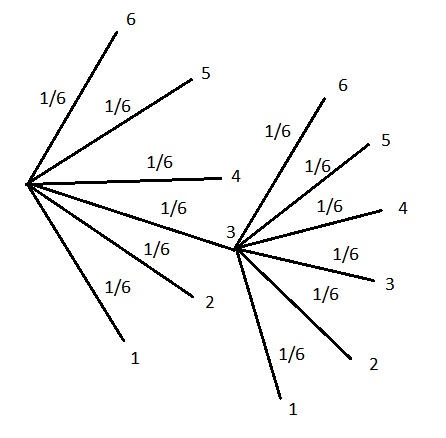
\includegraphics{problema15}\\
    P(7\geq) = \frac{1}{6}[\frac{1}{6}(1+2+3+4+5+6)]=\frac{21}{36}\\
    P(9) = \frac{4}{36}\\
    P(9|7\geq) = \frac{P(9|7\geq)}{P(7\geq)} = \frac{\frac{4}{36}}{\frac{21}{36}} = \frac{4}{21}\text{ ó } 19.04\%
    \end{gather*}
    \item Supongamos que 5 de cada 100 hombres y 25 de cada 10000 sufren daltonismo.\\
    Una persona daltónica se escoge aleatoriamente.\\
    ¿Cuál es la probabilidad de que sea hombre? (Supongamos que hay el mismo número de hombres que de mujeres)
    \\\textbf{Solución}
    \begin{gather*}
    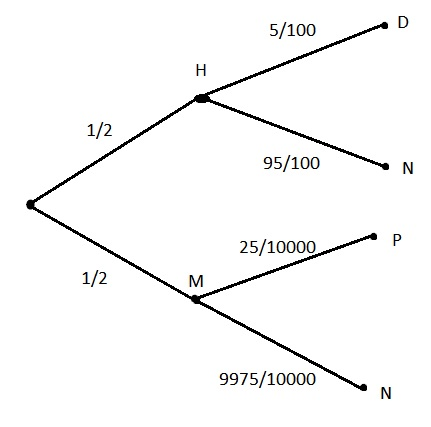
\includegraphics{problema16}\\
    P(D) = (\frac{1}{2})(\frac{5}{100})+(\frac{1}{2})(\frac{25}{10000})=\frac{525}{20000}\\
    P(H|D) = \frac{P(H \cap D)}{P(D)} = \frac{\frac{500}{20000}}{\frac{525}{20000}} = \frac{500}{525} = \frac{20}{21} \text{ ó } 95.23\%
    \end{gather*}
    \item Se escoge al azar un punto entre el 0 y el 1 en el eje de las x dentro del plano(x,y).\\A continuación se dibuja un circulo con centro en el origen y radio determinado por el punto escogido.\\Calcula la probabilidad de que el área del circulo sea menor que $\pi$/2
    \\\textbf{Solución}
    \begin{gather*}
    \pi r^{2}=\frac{\pi}{2}\\
    r=\frac{1}{\sqrt{2}}\\
    p(A) = \frac{\frac{1}{\sqrt{2}}}{1}=\frac{1}{\sqrt{2}} \text{ ó } 70.71\%
    \end{gather*}
    \item Se rompe una regla de 12 pulgadas al azar en 2 partes a lo largo.\\
    ¿Cuál es la probabilidad de que la longitud de la parte más larga sea al menos el doble de la corta?
    \\\textbf{Solución}
    \begin{gather*}
    x + y = 12\\
    y = \frac{x}{2}\\
    x + \frac{x}{2} = 12\\
    x = 8\\
    L = 12 - 8 = 4*2 = 8\\
    P(L)=\frac{8}{12}=\frac{2}{3}
    \end{gather*}
    \item Si la función de probabilidad de la variable aleatoria y esta dada por:
    \begin{gather*}
    f(y)= \left\{ \begin{array}{lcc}
    \frac{1}{8}(y+1) & 2 \leq y \leq 4\\
    \\ 0 & otro 
    \end{array}
    \right.
    \end{gather*}
    \\\textbf{Solución}
    \\\text{La variable es continua}
    \begin{gather*}
    P(\Omega)=1\\ 
    \end{gather*}
    \[ \int_{2}^{4}  \! F(y) \, dy =
    \int_{2}^{4}  \! \frac{1}{8}(y+1) \, dy =\frac{1}{8}\int_{2}^{4}  \! (y+1) \, dy = 
    \]
    \begin{gather*}
    \frac{1}{8}(\frac{y^2}{2}+y)|_2^4 =
    \frac{1}{8}[(8+4)-(2+2)]\frac{1}{8}(8)=1 \\
    \end{gather*}
    \\\textbf{Determine}\\
    \begin{enumerate}
        \item P(y $<$ 3.2)\\
        \item P(2.9 $<$ y $<$ 3.1)
    \end{enumerate}
    \begin{enumerate}
        \item  \[\frac{1}{8}\int_{2}^{3.2}  \! (y+1) \, dy =\frac{1}{8}(\frac{y^2}{2}+y)|_2^3.2 = \frac{1}{8}[(5.12+3.2)-(2+2)]=\frac{1}{8}[8.32-4]
        \]
        \[=\frac{4.32}{8}=54\% 
        \]
        \item \[\frac{1}{8}\int_{2.9}^{3.2}  \! (y+1) \, dy =\frac{1}{8}(\frac{y^2}{2}+y)|_2.9^3.2 = \frac{1}{8}[(5.12+3.2)-(4.205+2.9)]
        \]
        \[=\frac{1}{8}[1.215]=15.1875\% 
        \]
    \end{enumerate}
    \item Si la función de distribución de la variable aleatoria x está dada por
    \begin{gather*}
    f(y)= \left\{ \begin{array}{lcc}
    \frac{c}{\sqrt{x}} & 0 \leq x \leq 4\\
    \\ 0 & otro 
    \end{array}
    \right.
    \end{gather*}
    Determine el valor de c\\
    \\\textbf{Solución}
    \\\text{La variable es continua}
    \begin{gather*}
    P(\Omega)=1\\ 
    \end{gather*}
    \[ \int_{0}^{4}  \! \frac{c}{\sqrt{x}} \, dx =
    c\int_{0}^{4}  \! \frac{1}{\sqrt{x}} \, dx 
    \]
    "No se puede integrar"
    \[ \frac{1}{\sqrt{0}}
    \] No existe
    \item La cantidad real de café (en gramos) en un recipiente de 230 gr llenado por cierta máquina es una variable aleatoria cuya densidad de probabilidad está dada por
    \begin{gather*}
    f(y)= \left\{ \begin{array}{lcc}
    0 & x \leq 227.5\\
    \\ \frac{1}{5} & 227.5 < x < 232.5 \\
    \\ 0 & x \geq 232.5
    \end{array}
    \right.
    \end{gather*}
    Determine la probabilidad de que en un recipiente de 230gr llenado por esta máquina contendrá cuando mucho 228.65gr de café
    \\\textbf{Solución}
    \\\text{La variable es continua}
    \begin{gather*}
    P(\Omega)=1\\ 
    \end{gather*}
    \[ \int_{227.5}^{232.5}  \! \frac{1}{5} \, dx =
    \frac{1}{5}\int_{227.5}^{232.5}  \! \frac{1}{5} \, dx = \frac{1}{5}x |_{227.5}^{232.5}
    \] 
    \begin{gather*}
    \frac{5}{5}=1
    \end{gather*}
    \[ \int_{227.5}^{228.65}  \! \frac{1}{5} \, dx = \frac{1}{5}x |_{227.5}^{228.65} = \frac{1}{5}(228.65-227.5)
    \] 
    \[=\frac{1}{5}(1.15)= 0.23 \text{ ó} 23\% 
    \]
    % Para que empiece en 22
    \item El retraso o adelanto (en minutos) de un vuelo de Guadalajara a Monterrey es una variable aleatoria cuya densidad de probabilidad esta dada por: \\
    \begin{align*}
    f(x)= \left\{ \begin{array}{lcc}
    \frac{1}{288}(36 - x^2) &   si  & -6 \leq x \leq 6 \\
    \\ 0 &  ,  & DOM
    \end{array}
    \right.
    \end{align*}
    Donde los valores negativos son indicativos de que el vuelo llega adelantado y los valores positivos señalan que el vuelo llega retrasado. Determine la probabilidad de que uno de estos vuelos llegará cuando menos dos minutos antes.
    \\\textbf{Solución}
    \\\text{La variable es aleatoria continua.} \\
    \begin{gather*}
    P(\Omega) = 1 \\
    \frac{1}{288} \int \limits_{-6}^{6} (136-x^2) dx 
    = \frac{1}{288}(36x - \frac{x^3}{3})  \bigg\vert_{-6}^6 = \frac{1}{288}(216 - 72 + 216 - 72) \\		
    = \frac{1}{288}(288) = 1 \\
    \frac{1}{288} \int \limits_{-6}^{6} (136-x^2) dx 
    = \frac{1}{288}(36x - \frac{x^3}{3})  \bigg\vert_{-2}^{-6} = \frac{1}{288}(-72 + \frac{8}{3} + 216 - 72) = \frac{1}{288}(\frac{224}{3}) = 0.2592 \\
    \end{gather*}
    
    \item Si la ganancia de un contratista en una obra de construcción puede considerarse como una variable aleatoria que tiene la densidad de probabilidad: \\
    \begin{align*}
    f(x)= \left\{ \begin{array}{lcc}
    \frac{1}{18}(x + 1) &   si  & -1 \leq x \leq 5 \\
    \\ 0 &  ,  & DOM
    \end{array}
    \right.
    \end{align*}
    Donde las utilidades se expresan en miles de pesos, ¿cuál es la utilidad esperada?
    \\\textbf{Solución}
    \\\text{La variable es aleatoria continua.} \\
    \begin{gather*}
    \frac{1}{18} \int \limits_{-1}^{5} (x+1) dx = \frac{1}{18}(\frac{x^2}{2} + x) \bigg\vert_{-1}^5 = \frac{1}{18}(\frac{25}{2} + 5 - \frac{1}{2} + 1) = 1 \\
    \mu = \frac{1}{18} \int \limits_{-1}^{5} x(x+1) dx = \frac{1}{18}(\frac{x^3}{3} + \frac{x^2}{2}) \bigg\vert_{-1}^5 = 3 \\
    \end{gather*}
    Por lo tanto, la utilidad esperada es de 3. \\
    
    \item La probabilidad de que la Sra. Matínez venda una cadena de oro con una ganancia de \$3000 es: $ \frac{3}{20} $ . La probabilidad de que la venda y obtenga una ganancia de \$1500 es de $ \frac{7}{20} $ , la probabilidad de que salga a mano es $ \frac{7}{20} $ y la probabilidad de que pierda \$1500 es $ \frac{3}{20} $ . ¿Cuál es su ganancia esperada?
    \\\textbf{Solución}
    \\\text{La variable es aleatoria discreta, así:} \\
    \begin{gather*}
    \mu = \sum_{i = 0}^{n = 4} x_{i}f(x_{i}) = 3000*\frac{3}{20} + 1500*\frac{7}{20} + 0*\frac{7}{20} - 1500*\frac{3}{20} = 750 \\
    \end{gather*}
    Por lo tanto, su ganancia esperada es de \$750. \\
    
    \item El tiempo que tardan en atender a un individuo en una cafetería es una variable aleatoria con la densidad de probabilidad: \\
    \begin{align*}
    f(x)= \left\{ \begin{array}{lcc}
    \frac{1}{4}(e^{-\frac{x}{4}}) &   si  & x > 0 \\
    \\ 0 &  ,  & DOM
    \end{array}
    \right.
    \end{align*}
    Obtenga el valor esperado de esta distribución.
    \\\textbf{Solución}
    \\\text{La variable es aleatoria continua.} \\
    \begin{gather*}
    P(\Omega) = \int \limits_{0}^\infty (\frac{1}{4}(e^{-\frac{x}{4}})) dx = -e^{-\frac{x}{4}} \bigg\vert_{0}^{b} = \lim \limits_{b \rightarrow \infty} -e^{-\frac{b}{4}} - (-e^{0}) = 1 \\
    \mu = \int \limits_{0}^\infty (\frac{1}{4}x(e^{-\frac{x}{4}})) dx = \frac{1}{4}(e^{-\frac{x}{4}})(-4x-16) \bigg\vert_{0}^b = \lim \limits_{b \rightarrow \infty} -e^{-\frac{b}{4}}(-4b -16) - (-e^{0})(-16) = 4 \\
    \end{gather*}
    Por lo tanto el valor esperado es 4. \\
    
    \item El número de horas de operación satisfactoria que proporciona un televisor Sonny es una variable aleatoria de z cuya función de probabilidad es: \\
    \begin{align*}
    f(z)= \left\{ \begin{array}{lcc}
    0.0001e^{-0.0001z} &   si  & z > 0 \\
    \\ 0 &  ,  & DOM
    \end{array}
    \right.
    \end{align*}
    Obtenga el valor esperado de esta distribución.
    \\\textbf{Solución}
    \\\text{La variable es aleatoria continua.} \\
    \begin{gather*}
    P(\Omega) = \int \limits_{0}^{\infty} (0.0001e^{-0.0001z}) dz = -e^{-0.0001z} \bigg\vert_{0}^{b} = \lim \limits_{b \rightarrow \infty} -e^{-0.0001b} - (-e^{0}) = 1 \\
    \mu = \int \limits_{0}^{\infty} (0.0001ze^{-0.0001z}) dz = \frac{e{-\frac{x}{10 000}}(-10 000x - 100 000 000)}{10 000} \bigg\vert_{0}^b \\
    = \lim \limits_{b \rightarrow \infty} \frac{e{-\frac{b}{10 000}}(-10 000b - 100 000 000)}{10 000} - \frac{e{-\frac{0}{10 000}}(-10 000(0) - 100 000 000)}{10 000} = 10 000
    \end{gather*}
    Por lo tanto, el valor esperado es 10 000.
    
\end{enumerate}